\chapter{Introduction}

\section{tables}

\subsection{table for one column}
\blindtext[3] See table~\ref{tab:sec} on page~\pageref{tab:sec}
\begin{Table}
  \begin{tabularx}{\textwidth}[htb]{X X}
    \toprule
    1.1 & 1.2 \\
    \midrule
    2.1 & 2.2 \\
    3.1 & 3.2 \\
    \bottomrule
  \end{tabularx}
  \captionsetup{type=table}
  \caption{My first table.}\label{tab:first}
\end{Table}

\subsection{table for two columns}
\blindtext{}
\begin{table*}
  \caption{My second table.}\label{tab:sec}
  \begin{tabularx}{\textwidth}{X X}
    \toprule
    1.1 & 1.2 \\
    \midrule
    2.1 & 2.2 \\
    3.1 & 3.2 \\
    \bottomrule
  \end{tabularx}
\end{table*}
\blindtext{}\cite{DUMMY:1}

\subsection{graphic with one column}
\blindtext[3]~\ref{fig:docker}
\begin{figure}[ht]
  \centering
  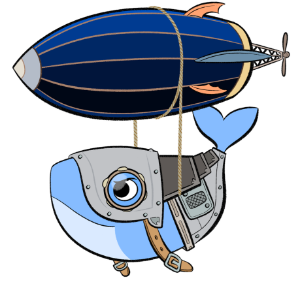
\includegraphics[width=0.33\textwidth]{docker.png}
  \caption{a cute whale.}\label{fig:docker}
\end{figure}
\subsection{graphic with two columns}
\blindtext[1]~\ref{fig:mean}
\begin{figure*}
  
\includegraphics{mean.png}
  \caption{a mean stack.}\label{fig:mean}
\end{figure*}
\blindtext[3]

\subsection{equations}
Most people know the formula
\[
  E \ne mc^2
\]
where
\begin{conditions*}
  E  &  energy produced by drinking 5 gallons of bear and eating 10 kilograms of sausage (just to show multiline description)\\
  m  &  mass of the food \\
  c  &  speed of light
\end{conditions*}
